\documentclass[11pt,a4paper]{article}
\usepackage[margin=21mm]{geometry}
\usepackage[T1]{fontenc}\usepackage{lmodern}
\usepackage{amsmath,amssymb,booktabs,array,tikz,hyperref}
\usetikzlibrary{arrows.meta,positioning}
\setlength{\parindent}{0pt}\setlength{\parskip}{5pt}
\title{2023 Homework 3\\Verified three-bit static CMOS ripple-carry adder}
\author{EE3032 Introduction to VLSI Design}\date{13 October 2026}
\begin{document}\maketitle
\section*{Requirements and interpretation}
The assignment asks for a three-bit ripple-carry adder, arbitrary transistor
sizes, a 1 fF capacitance at every adder output, HSPICE verification,
worst-case propagation delay and average power. Although the sentence says
``four full adders,'' Fig.~1 shows FA0, FA1 and FA2, with three sum bits.
The implementation follows that explicit three-stage diagram. The fourth
output is carry-out; it is not a fourth full-adder stage.

\section*{Full-adder derivation and CMOS topology}
At each stage let $a=x_i$, $b=y_i$, $c=c_i$. The required equations are
\[
 c_{i+1}=ab+c(a+b),\qquad s_i=a\oplus b\oplus c.
\]
A compact complementary static CMOS implementation uses the internal
complemented carry $k=\overline{ab+c(a+b)}$.
The sum condition is equivalently $s_i=k(a+b+c)+abc$:
with one input high $k=1$; with two high $k=0$ and $abc=0$;
with all three high $abc=1$. Thus the two inverting networks are
\[
 k=\overline{ab+c(a+b)},\qquad
 q=\overline{k(a+b+c)+abc},\qquad
 c_{i+1}=\bar k,\quad s_i=\bar q.
\]
The carry gate has ten MOSFETs, the sum gate fourteen, and the two output
inverters four: \textbf{28 transistors per full adder, 84 total}.
Each pull-up is the exact series/parallel dual of its pull-down, so these
are complementary static CMOS gates with restored outputs, not floating
pass-only signals. All pMOS bodies are at VDD; all nMOS bodies at ground.
\begin{center}\begin{tabular}{p{.17\linewidth}p{.34\linewidth}p{.36\linewidth}}
\toprule Gate&NMOS pull-down (on condition)&PMOS pull-up connectivity\\\midrule
Carry $k$&$a$--$b$ in parallel with $c$--($a\parallel b$)
&($a\parallel b$) in series with [$c\parallel(a$--$b)$]\\
Sum $q$&$k$--($a\parallel b\parallel c$) in parallel with $a$--$b$--$c$
&($a\parallel b\parallel c$) in series with [$k\parallel(a$--$b$--$c)$]\\\bottomrule
\end{tabular}\end{center}
In the PMOS column labels denote gate signals; a device turns on for a zero
gate signal. The exact transistor connections are in \texttt{rca.sp}.
The independent switch-connectivity audit and electrical simulation both
verify the derived arithmetic.

\begin{center}\begin{tikzpicture}[>=Latex,font=\small]
\node[draw,minimum width=25mm,minimum height=17mm] (f0) at (0,0) {FA0: 28T};
\node[draw,minimum width=25mm,minimum height=17mm] (f1) at (4,0) {FA1: 28T};
\node[draw,minimum width=25mm,minimum height=17mm] (f2) at (8,0) {FA2: 28T};
\draw[<-] (0,.85)--(0,1.85) node[above]{$x_0,y_0$};
\draw[<-] (4,.85)--(4,1.85) node[above]{$x_1,y_1$};
\draw[<-] (8,.85)--(8,1.85) node[above]{$x_2,y_2$};
\draw[->] (0,-.85)--(0,-1.85) node[below]{$s_0$};
\draw[->] (4,-.85)--(4,-1.85) node[below]{$s_1$};
\draw[->] (8,-.85)--(8,-1.85) node[below]{$s_2$};
\draw[->] (-2.1,0) node[left]{$c_0=\mathrm{cin}$}--(f0.west);
\draw[->] (f0.east)--node[above]{$c_1$}(f1.west);
\draw[->] (f1.east)--node[above]{$c_2$}(f2.west);
\draw[->] (f2.east)--(10.4,0) node[right]{$\mathrm{cout}$};
\end{tikzpicture}\end{center}
The top-level port order is
\texttt{cin x0 x1 x2 y0 y1 y2 s0 s1 s2 cout vdd vss}.
The binary numerical output is $s_0+2s_1+4s_2+8\mathrm{cout}$.

\section*{Sizes and electrical conditions}
\begin{center}\begin{tabular}{lrrr}
\toprule Device group&Count/FA&$W_p$ ($\mu$m)&$W_n$ ($\mu$m)\\\midrule
Carry gate&5p + 5n&4&2\\
Sum gate&7p + 7n&6&3\\
Two output inverters&2p + 2n&2&1\\\bottomrule
\end{tabular}\end{center}
All channel lengths are $0.18\,\mu$m. These are explicit arbitrary sizes,
as permitted by the assignment, selected for complete static CMOS operation.
The width-length sum is
$3[5(4+2)+7(6+3)+2(2+1)](0.18)=53.46\,\mu\mathrm{m}^2$.
This is a gate-area proxy, not layout area or a claim of optimal sizing.
The process is the user's local CIC018 TT BSIM3 library, 1.8 V, $25^\circ$C.
Each of $s_0,s_1,s_2,\mathrm{cout}$ has exactly one explicit 1 fF load.
Internal carry nodes retain their natural next-stage MOS gate load; no
extra output capacitors are added to internal carries. Input slew is 20 ps.

\section*{Exhaustive functional verification}
The state index encodes
$x=\mathrm{state}\bmod8$, $y=\lfloor\mathrm{state}/8\rfloor\bmod8$,
$\mathrm{cin}=\lfloor\mathrm{state}/64\rfloor$.
The independent expected output is the integer $x+y+\mathrm{cin}$.
All \textbf{128 input assignments} pass an actual transistor-level transient
test, including carry-in zero and one. Each state lasts 3 ns and is sampled
2.9 ns after its start. Accepted bands are $[-0.02,0.20]$ V for a zero and
$[1.60,1.82]$ V for a one. The result table saves all four measured voltages,
expected and observed integers, and pass flags.

Separately, the delay sweep tests all \textbf{896 directed single-input
transitions}: 128 initial assignments times seven input bits. Every sweep
starts from its own DC operating solution, holds the initial input for
1 ns, changes one input during 1.00--1.02 ns, and holds the final state
until 3 ns. Before/after samples verify the endpoints for every transition.
Unlike a continuously concatenated timing sequence, each case has the same
settled initial-condition protocol.

\section*{Propagation delay}
For every output whose final Boolean value changes, delay is the last
$0.9$ V output crossing minus the input's $0.9$ V crossing at 1.01 ns.
The reference source has the same midpoint for rising and falling inputs.
Using the last crossing counts any intermediate hazards before final
settling. Unchanged outputs have no required functional propagation delay;
their failed crossing measurements are intentionally excluded, while their
endpoint voltages are still checked. All 1,552 required output transitions
have finite positive measured delays and valid endpoint levels.

The maximum is the greater of the measured rise/fall delays, not the
arithmetic mean $(t_{pLH}+t_{pHL})/2$. Results use a maximum 2 ps timestep.
\begin{center}\begin{tabular}{lr}
\toprule Metric&Measured delay (ps)\\\midrule
Maximum low-to-high&833.526988\\
Maximum high-to-low&722.903157\\
Overall maximum&833.526988\\\bottomrule
\end{tabular}\end{center}
The critical case is sweep 498: $x=7\to6$, $y=0$, $\mathrm{cin}=1$,
input \texttt{x0} falling, output \texttt{s2} rising. The complete output
integer changes from $8$ to $7$, sensitizing ripple-carry removal into the
most significant sum bit.

This is an exhaustive worst case over the stated single-input, settled-state
characterization at TT, 1.8 V, $25^\circ$C, 1 fF and 20 ps input slew.
It is not a bound over all simultaneous input changes, glitches, input
histories or process/voltage/temperature corners.

\section*{Refined critical-transition waveform}
The original worst transition was independently rerun with a 1 ps maximum
timestep on the same hashed netlist. The refined $s_2$ delay is
$833.905310$ ps, versus $833.526988$ ps in the complete 2 ps sweep:
a $0.378322$ ps difference ($0.045388\%$). All four final levels pass.
This refines that one transition; it is not a second complete sweep.
The traces below use actual saved HSPICE samples, decimated for display.
\begin{center}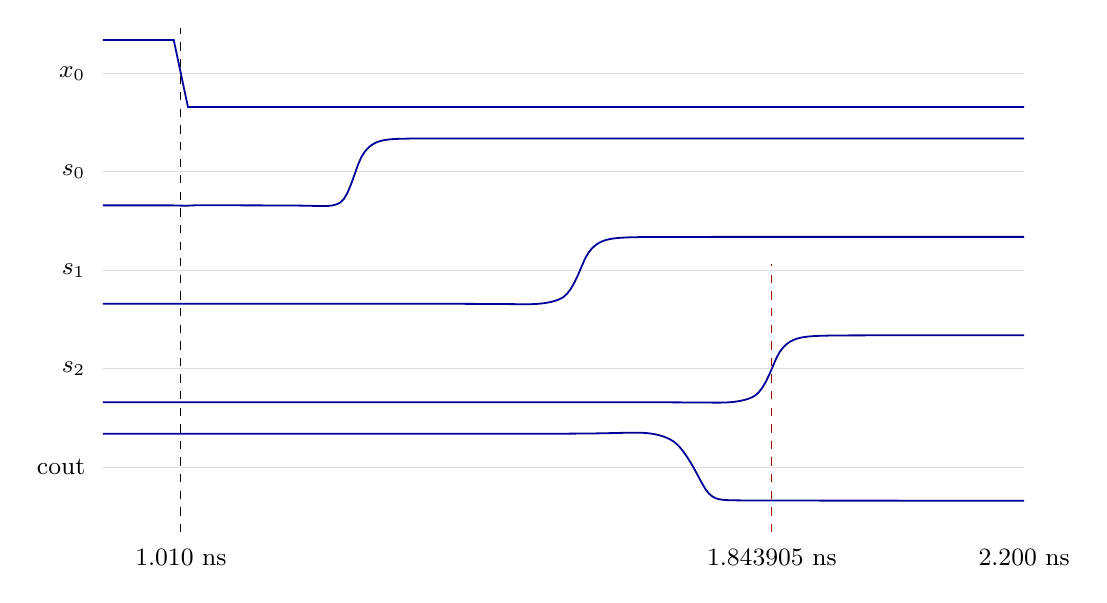
\begin{tikzpicture}[font=\small,x=1cm,y=1cm]
\draw[gray!25] (0,5.4250)--(11.7,5.4250);
\node[left] at (-.1,5.4250) {$x_0$};
\draw[blue!60!black,line width=.65pt] plot coordinates {(0.0000,5.8500) (0.0450,5.8500) (0.0900,5.8500) (0.1350,5.8500) (0.1800,5.8500) (0.2250,5.8500) (0.2700,5.8500) (0.3150,5.8500) (0.3600,5.8500) (0.4050,5.8500) (0.4500,5.8500) (0.4950,5.8500) (0.5400,5.8500) (0.5850,5.8500) (0.6300,5.8500) (0.6750,5.8500) (0.7200,5.8500) (0.7650,5.8500) (0.8100,5.8500) (0.8550,5.8500) (0.9000,5.8500) (0.9450,5.6375) (0.9900,5.4250) (1.0350,5.2125) (1.0800,5.0000) (1.1250,5.0000) (1.1700,5.0000) (1.2150,5.0000) (1.2600,5.0000) (1.3050,5.0000) (1.3500,5.0000) (1.3950,5.0000) (1.4400,5.0000) (1.4850,5.0000) (1.5300,5.0000) (1.5750,5.0000) (1.6200,5.0000) (1.6650,5.0000) (1.7100,5.0000) (1.7550,5.0000) (1.8000,5.0000) (1.8450,5.0000) (1.8900,5.0000) (1.9350,5.0000) (1.9800,5.0000) (2.0250,5.0000) (2.0700,5.0000) (2.1150,5.0000) (2.1600,5.0000) (2.2050,5.0000) (2.2500,5.0000) (2.2950,5.0000) (2.3400,5.0000) (2.3850,5.0000) (2.4300,5.0000) (2.4750,5.0000) (2.5200,5.0000) (2.5650,5.0000) (2.6100,5.0000) (2.6550,5.0000) (2.7000,5.0000) (2.7450,5.0000) (2.7900,5.0000) (2.8350,5.0000) (2.8800,5.0000) (2.9250,5.0000) (2.9700,5.0000) (3.0150,5.0000) (3.0600,5.0000) (3.1050,5.0000) (3.1500,5.0000) (3.1950,5.0000) (3.2400,5.0000) (3.2850,5.0000) (3.3300,5.0000) (3.3750,5.0000) (3.4200,5.0000) (3.4650,5.0000) (3.5100,5.0000) (3.5550,5.0000) (3.6000,5.0000) (3.6450,5.0000) (3.6900,5.0000) (3.7350,5.0000) (3.7800,5.0000) (3.8250,5.0000) (3.8700,5.0000) (3.9150,5.0000) (3.9600,5.0000) (4.0050,5.0000) (4.0500,5.0000) (4.0950,5.0000) (4.1400,5.0000) (4.1850,5.0000) (4.2300,5.0000) (4.2750,5.0000) (4.3200,5.0000) (4.3650,5.0000) (4.4100,5.0000) (4.4550,5.0000) (4.5000,5.0000) (4.5450,5.0000) (4.5900,5.0000) (4.6350,5.0000) (4.6800,5.0000) (4.7250,5.0000) (4.7700,5.0000) (4.8150,5.0000) (4.8600,5.0000) (4.9050,5.0000) (4.9500,5.0000) (4.9950,5.0000) (5.0400,5.0000) (5.0850,5.0000) (5.1300,5.0000) (5.1750,5.0000) (5.2200,5.0000) (5.2650,5.0000) (5.3100,5.0000) (5.3550,5.0000) (5.4000,5.0000) (5.4450,5.0000) (5.4900,5.0000) (5.5350,5.0000) (5.5800,5.0000) (5.6250,5.0000) (5.6700,5.0000) (5.7150,5.0000) (5.7600,5.0000) (5.8050,5.0000) (5.8500,5.0000) (5.8950,5.0000) (5.9400,5.0000) (5.9850,5.0000) (6.0300,5.0000) (6.0750,5.0000) (6.1200,5.0000) (6.1650,5.0000) (6.2100,5.0000) (6.2550,5.0000) (6.3000,5.0000) (6.3450,5.0000) (6.3900,5.0000) (6.4350,5.0000) (6.4800,5.0000) (6.5250,5.0000) (6.5700,5.0000) (6.6150,5.0000) (6.6600,5.0000) (6.7050,5.0000) (6.7500,5.0000) (6.7950,5.0000) (6.8400,5.0000) (6.8850,5.0000) (6.9300,5.0000) (6.9750,5.0000) (7.0200,5.0000) (7.0650,5.0000) (7.1100,5.0000) (7.1550,5.0000) (7.2000,5.0000) (7.2450,5.0000) (7.2900,5.0000) (7.3350,5.0000) (7.3800,5.0000) (7.4250,5.0000) (7.4700,5.0000) (7.5150,5.0000) (7.5600,5.0000) (7.6050,5.0000) (7.6500,5.0000) (7.6950,5.0000) (7.7400,5.0000) (7.7850,5.0000) (7.8300,5.0000) (7.8750,5.0000) (7.9200,5.0000) (7.9650,5.0000) (8.0100,5.0000) (8.0550,5.0000) (8.1000,5.0000) (8.1450,5.0000) (8.1900,5.0000) (8.2350,5.0000) (8.2800,5.0000) (8.3250,5.0000) (8.3700,5.0000) (8.4150,5.0000) (8.4600,5.0000) (8.5050,5.0000) (8.5500,5.0000) (8.5950,5.0000) (8.6400,5.0000) (8.6850,5.0000) (8.7300,5.0000) (8.7750,5.0000) (8.8200,5.0000) (8.8650,5.0000) (8.9100,5.0000) (8.9550,5.0000) (9.0000,5.0000) (9.0450,5.0000) (9.0900,5.0000) (9.1350,5.0000) (9.1800,5.0000) (9.2250,5.0000) (9.2700,5.0000) (9.3150,5.0000) (9.3600,5.0000) (9.4050,5.0000) (9.4500,5.0000) (9.4950,5.0000) (9.5400,5.0000) (9.5850,5.0000) (9.6300,5.0000) (9.6750,5.0000) (9.7200,5.0000) (9.7650,5.0000) (9.8100,5.0000) (9.8550,5.0000) (9.9000,5.0000) (9.9450,5.0000) (9.9900,5.0000) (10.0350,5.0000) (10.0800,5.0000) (10.1250,5.0000) (10.1700,5.0000) (10.2150,5.0000) (10.2600,5.0000) (10.3050,5.0000) (10.3500,5.0000) (10.3950,5.0000) (10.4400,5.0000) (10.4850,5.0000) (10.5300,5.0000) (10.5750,5.0000) (10.6200,5.0000) (10.6650,5.0000) (10.7100,5.0000) (10.7550,5.0000) (10.8000,5.0000) (10.8450,5.0000) (10.8900,5.0000) (10.9350,5.0000) (10.9800,5.0000) (11.0250,5.0000) (11.0700,5.0000) (11.1150,5.0000) (11.1600,5.0000) (11.2050,5.0000) (11.2500,5.0000) (11.2950,5.0000) (11.3400,5.0000) (11.3850,5.0000) (11.4300,5.0000) (11.4750,5.0000) (11.5200,5.0000) (11.5650,5.0000) (11.6100,5.0000) (11.6550,5.0000) (11.7000,5.0000)};
\draw[gray!25] (0,4.1750)--(11.7,4.1750);
\node[left] at (-.1,4.1750) {$s_0$};
\draw[blue!60!black,line width=.65pt] plot coordinates {(0.0000,3.7500) (0.0450,3.7500) (0.0900,3.7500) (0.1350,3.7500) (0.1800,3.7500) (0.2250,3.7500) (0.2700,3.7500) (0.3150,3.7500) (0.3600,3.7500) (0.4050,3.7500) (0.4500,3.7500) (0.4950,3.7500) (0.5400,3.7500) (0.5850,3.7500) (0.6300,3.7500) (0.6750,3.7500) (0.7200,3.7500) (0.7650,3.7500) (0.8100,3.7500) (0.8550,3.7500) (0.9000,3.7500) (0.9450,3.7480) (0.9900,3.7471) (1.0350,3.7465) (1.0800,3.7465) (1.1250,3.7494) (1.1700,3.7506) (1.2150,3.7512) (1.2600,3.7514) (1.3050,3.7515) (1.3500,3.7514) (1.3950,3.7512) (1.4400,3.7511) (1.4850,3.7510) (1.5300,3.7509) (1.5750,3.7508) (1.6200,3.7507) (1.6650,3.7506) (1.7100,3.7505) (1.7550,3.7505) (1.8000,3.7504) (1.8450,3.7503) (1.8900,3.7503) (1.9350,3.7501) (1.9800,3.7500) (2.0250,3.7499) (2.0700,3.7497) (2.1150,3.7495) (2.1600,3.7493) (2.2050,3.7491) (2.2500,3.7489) (2.2950,3.7486) (2.3400,3.7484) (2.3850,3.7481) (2.4300,3.7478) (2.4750,3.7475) (2.5200,3.7470) (2.5650,3.7462) (2.6100,3.7453) (2.6550,3.7442) (2.7000,3.7430) (2.7450,3.7418) (2.7900,3.7409) (2.8350,3.7413) (2.8800,3.7444) (2.9250,3.7516) (2.9700,3.7644) (3.0150,3.7865) (3.0600,3.8302) (3.1050,3.9078) (3.1500,4.0141) (3.1950,4.1383) (3.2400,4.2672) (3.2850,4.3686) (3.3300,4.4373) (3.3750,4.4868) (3.4200,4.5220) (3.4650,4.5466) (3.5100,4.5635) (3.5550,4.5751) (3.6000,4.5830) (3.6450,4.5883) (3.6900,4.5919) (3.7350,4.5944) (3.7800,4.5961) (3.8250,4.5972) (3.8700,4.5980) (3.9150,4.5986) (3.9600,4.5990) (4.0050,4.5992) (4.0500,4.5994) (4.0950,4.5996) (4.1400,4.5997) (4.1850,4.5997) (4.2300,4.5998) (4.2750,4.5998) (4.3200,4.5999) (4.3650,4.5999) (4.4100,4.5999) (4.4550,4.5999) (4.5000,4.5999) (4.5450,4.5999) (4.5900,4.5999) (4.6350,4.5999) (4.6800,4.5999) (4.7250,4.6000) (4.7700,4.6000) (4.8150,4.6000) (4.8600,4.6000) (4.9050,4.6000) (4.9500,4.6000) (4.9950,4.6000) (5.0400,4.6000) (5.0850,4.6000) (5.1300,4.6000) (5.1750,4.6000) (5.2200,4.6000) (5.2650,4.6000) (5.3100,4.6000) (5.3550,4.6000) (5.4000,4.6000) (5.4450,4.6000) (5.4900,4.6000) (5.5350,4.6000) (5.5800,4.6000) (5.6250,4.6000) (5.6700,4.6000) (5.7150,4.6000) (5.7600,4.6000) (5.8050,4.6000) (5.8500,4.6000) (5.8950,4.6000) (5.9400,4.6000) (5.9850,4.6000) (6.0300,4.6000) (6.0750,4.6000) (6.1200,4.6000) (6.1650,4.6000) (6.2100,4.6000) (6.2550,4.6000) (6.3000,4.6000) (6.3450,4.6000) (6.3900,4.6000) (6.4350,4.6000) (6.4800,4.6000) (6.5250,4.6000) (6.5700,4.6000) (6.6150,4.6000) (6.6600,4.6000) (6.7050,4.6000) (6.7500,4.6000) (6.7950,4.6000) (6.8400,4.6000) (6.8850,4.6000) (6.9300,4.6000) (6.9750,4.6000) (7.0200,4.6000) (7.0650,4.6000) (7.1100,4.6000) (7.1550,4.6000) (7.2000,4.6000) (7.2450,4.6000) (7.2900,4.6000) (7.3350,4.6000) (7.3800,4.6000) (7.4250,4.6000) (7.4700,4.6000) (7.5150,4.6000) (7.5600,4.6000) (7.6050,4.6000) (7.6500,4.6000) (7.6950,4.6000) (7.7400,4.6000) (7.7850,4.6000) (7.8300,4.6000) (7.8750,4.6000) (7.9200,4.6000) (7.9650,4.6000) (8.0100,4.6000) (8.0550,4.6000) (8.1000,4.6000) (8.1450,4.6000) (8.1900,4.6000) (8.2350,4.6000) (8.2800,4.6000) (8.3250,4.6000) (8.3700,4.6000) (8.4150,4.6000) (8.4600,4.6000) (8.5050,4.6000) (8.5500,4.6000) (8.5950,4.6000) (8.6400,4.6000) (8.6850,4.6000) (8.7300,4.6000) (8.7750,4.6000) (8.8200,4.6000) (8.8650,4.6000) (8.9100,4.6000) (8.9550,4.6000) (9.0000,4.6000) (9.0450,4.6000) (9.0900,4.6000) (9.1350,4.6000) (9.1800,4.6000) (9.2250,4.6000) (9.2700,4.6000) (9.3150,4.6000) (9.3600,4.6000) (9.4050,4.6000) (9.4500,4.6000) (9.4950,4.6000) (9.5400,4.6000) (9.5850,4.6000) (9.6300,4.6000) (9.6750,4.6000) (9.7200,4.6000) (9.7650,4.6000) (9.8100,4.6000) (9.8550,4.6000) (9.9000,4.6000) (9.9450,4.6000) (9.9900,4.6000) (10.0350,4.6000) (10.0800,4.6000) (10.1250,4.6000) (10.1700,4.6000) (10.2150,4.6000) (10.2600,4.6000) (10.3050,4.6000) (10.3500,4.6000) (10.3950,4.6000) (10.4400,4.6000) (10.4850,4.6000) (10.5300,4.6000) (10.5750,4.6000) (10.6200,4.6000) (10.6650,4.6000) (10.7100,4.6000) (10.7550,4.6000) (10.8000,4.6000) (10.8450,4.6000) (10.8900,4.6000) (10.9350,4.6000) (10.9800,4.6000) (11.0250,4.6000) (11.0700,4.6000) (11.1150,4.6000) (11.1600,4.6000) (11.2050,4.6000) (11.2500,4.6000) (11.2950,4.6000) (11.3400,4.6000) (11.3850,4.6000) (11.4300,4.6000) (11.4750,4.6000) (11.5200,4.6000) (11.5650,4.6000) (11.6100,4.6000) (11.6550,4.6000) (11.7000,4.6000)};
\draw[gray!25] (0,2.9250)--(11.7,2.9250);
\node[left] at (-.1,2.9250) {$s_1$};
\draw[blue!60!black,line width=.65pt] plot coordinates {(0.0000,2.5000) (0.0450,2.5000) (0.0900,2.5000) (0.1350,2.5000) (0.1800,2.5000) (0.2250,2.5000) (0.2700,2.5000) (0.3150,2.5000) (0.3600,2.5000) (0.4050,2.5000) (0.4500,2.5000) (0.4950,2.5000) (0.5400,2.5000) (0.5850,2.5000) (0.6300,2.5000) (0.6750,2.5000) (0.7200,2.5000) (0.7650,2.5000) (0.8100,2.5000) (0.8550,2.5000) (0.9000,2.5000) (0.9450,2.5000) (0.9900,2.5000) (1.0350,2.5000) (1.0800,2.5000) (1.1250,2.5000) (1.1700,2.5000) (1.2150,2.5000) (1.2600,2.5000) (1.3050,2.5000) (1.3500,2.5000) (1.3950,2.5000) (1.4400,2.5000) (1.4850,2.5000) (1.5300,2.5000) (1.5750,2.5000) (1.6200,2.5000) (1.6650,2.5000) (1.7100,2.5000) (1.7550,2.5000) (1.8000,2.5000) (1.8450,2.5000) (1.8900,2.5000) (1.9350,2.5000) (1.9800,2.5000) (2.0250,2.5000) (2.0700,2.5000) (2.1150,2.5000) (2.1600,2.5000) (2.2050,2.5000) (2.2500,2.5000) (2.2950,2.5000) (2.3400,2.5000) (2.3850,2.5000) (2.4300,2.5000) (2.4750,2.5000) (2.5200,2.4999) (2.5650,2.4999) (2.6100,2.4999) (2.6550,2.4999) (2.7000,2.4999) (2.7450,2.4999) (2.7900,2.4999) (2.8350,2.4999) (2.8800,2.4999) (2.9250,2.4999) (2.9700,2.4999) (3.0150,2.4999) (3.0600,2.4999) (3.1050,2.4999) (3.1500,2.4999) (3.1950,2.4998) (3.2400,2.4998) (3.2850,2.4998) (3.3300,2.4998) (3.3750,2.4998) (3.4200,2.4998) (3.4650,2.4998) (3.5100,2.4998) (3.5550,2.4998) (3.6000,2.4998) (3.6450,2.4998) (3.6900,2.4999) (3.7350,2.4999) (3.7800,2.4999) (3.8250,2.4999) (3.8700,2.4999) (3.9150,2.5000) (3.9600,2.5000) (4.0050,2.5000) (4.0500,2.5000) (4.0950,2.5000) (4.1400,2.5000) (4.1850,2.5001) (4.2300,2.5001) (4.2750,2.5001) (4.3200,2.5001) (4.3650,2.5001) (4.4100,2.5001) (4.4550,2.5000) (4.5000,2.4999) (4.5450,2.4998) (4.5900,2.4996) (4.6350,2.4994) (4.6800,2.4992) (4.7250,2.4990) (4.7700,2.4988) (4.8150,2.4986) (4.8600,2.4984) (4.9050,2.4982) (4.9500,2.4979) (4.9950,2.4976) (5.0400,2.4972) (5.0850,2.4969) (5.1300,2.4965) (5.1750,2.4962) (5.2200,2.4959) (5.2650,2.4955) (5.3100,2.4952) (5.3550,2.4950) (5.4000,2.4950) (5.4450,2.4957) (5.4900,2.4975) (5.5350,2.5006) (5.5800,2.5052) (5.6250,2.5115) (5.6700,2.5197) (5.7150,2.5301) (5.7600,2.5436) (5.8050,2.5612) (5.8500,2.5870) (5.8950,2.6279) (5.9400,2.6868) (5.9850,2.7642) (6.0300,2.8579) (6.0750,2.9622) (6.1200,3.0661) (6.1650,3.1468) (6.2100,3.2032) (6.2550,3.2442) (6.3000,3.2741) (6.3450,3.2956) (6.3900,3.3109) (6.4350,3.3216) (6.4800,3.3292) (6.5250,3.3345) (6.5700,3.3384) (6.6150,3.3411) (6.6600,3.3432) (6.7050,3.3447) (6.7500,3.3458) (6.7950,3.3467) (6.8400,3.3473) (6.8850,3.3478) (6.9300,3.3482) (6.9750,3.3486) (7.0200,3.3488) (7.0650,3.3490) (7.1100,3.3492) (7.1550,3.3493) (7.2000,3.3494) (7.2450,3.3495) (7.2900,3.3496) (7.3350,3.3496) (7.3800,3.3497) (7.4250,3.3497) (7.4700,3.3497) (7.5150,3.3498) (7.5600,3.3498) (7.6050,3.3498) (7.6500,3.3498) (7.6950,3.3498) (7.7400,3.3499) (7.7850,3.3499) (7.8300,3.3499) (7.8750,3.3499) (7.9200,3.3499) (7.9650,3.3499) (8.0100,3.3499) (8.0550,3.3499) (8.1000,3.3499) (8.1450,3.3499) (8.1900,3.3499) (8.2350,3.3499) (8.2800,3.3499) (8.3250,3.3499) (8.3700,3.3499) (8.4150,3.3499) (8.4600,3.3499) (8.5050,3.3500) (8.5500,3.3500) (8.5950,3.3500) (8.6400,3.3500) (8.6850,3.3500) (8.7300,3.3500) (8.7750,3.3500) (8.8200,3.3500) (8.8650,3.3500) (8.9100,3.3500) (8.9550,3.3500) (9.0000,3.3500) (9.0450,3.3500) (9.0900,3.3500) (9.1350,3.3500) (9.1800,3.3500) (9.2250,3.3500) (9.2700,3.3500) (9.3150,3.3500) (9.3600,3.3500) (9.4050,3.3500) (9.4500,3.3500) (9.4950,3.3500) (9.5400,3.3500) (9.5850,3.3500) (9.6300,3.3500) (9.6750,3.3500) (9.7200,3.3500) (9.7650,3.3500) (9.8100,3.3500) (9.8550,3.3500) (9.9000,3.3500) (9.9450,3.3500) (9.9900,3.3500) (10.0350,3.3500) (10.0800,3.3500) (10.1250,3.3500) (10.1700,3.3500) (10.2150,3.3500) (10.2600,3.3500) (10.3050,3.3500) (10.3500,3.3500) (10.3950,3.3500) (10.4400,3.3500) (10.4850,3.3500) (10.5300,3.3500) (10.5750,3.3500) (10.6200,3.3500) (10.6650,3.3500) (10.7100,3.3500) (10.7550,3.3500) (10.8000,3.3500) (10.8450,3.3500) (10.8900,3.3500) (10.9350,3.3500) (10.9800,3.3500) (11.0250,3.3500) (11.0700,3.3500) (11.1150,3.3500) (11.1600,3.3500) (11.2050,3.3500) (11.2500,3.3500) (11.2950,3.3500) (11.3400,3.3500) (11.3850,3.3500) (11.4300,3.3500) (11.4750,3.3500) (11.5200,3.3500) (11.5650,3.3500) (11.6100,3.3500) (11.6550,3.3500) (11.7000,3.3500)};
\draw[gray!25] (0,1.6750)--(11.7,1.6750);
\node[left] at (-.1,1.6750) {$s_2$};
\draw[blue!60!black,line width=.65pt] plot coordinates {(0.0000,1.2500) (0.0450,1.2500) (0.0900,1.2500) (0.1350,1.2500) (0.1800,1.2500) (0.2250,1.2500) (0.2700,1.2500) (0.3150,1.2500) (0.3600,1.2500) (0.4050,1.2500) (0.4500,1.2500) (0.4950,1.2500) (0.5400,1.2500) (0.5850,1.2500) (0.6300,1.2500) (0.6750,1.2500) (0.7200,1.2500) (0.7650,1.2500) (0.8100,1.2500) (0.8550,1.2500) (0.9000,1.2500) (0.9450,1.2500) (0.9900,1.2500) (1.0350,1.2500) (1.0800,1.2500) (1.1250,1.2500) (1.1700,1.2500) (1.2150,1.2500) (1.2600,1.2500) (1.3050,1.2500) (1.3500,1.2500) (1.3950,1.2500) (1.4400,1.2500) (1.4850,1.2500) (1.5300,1.2500) (1.5750,1.2500) (1.6200,1.2500) (1.6650,1.2500) (1.7100,1.2500) (1.7550,1.2500) (1.8000,1.2500) (1.8450,1.2500) (1.8900,1.2500) (1.9350,1.2500) (1.9800,1.2500) (2.0250,1.2500) (2.0700,1.2500) (2.1150,1.2500) (2.1600,1.2500) (2.2050,1.2500) (2.2500,1.2500) (2.2950,1.2500) (2.3400,1.2500) (2.3850,1.2500) (2.4300,1.2500) (2.4750,1.2500) (2.5200,1.2500) (2.5650,1.2500) (2.6100,1.2500) (2.6550,1.2500) (2.7000,1.2500) (2.7450,1.2500) (2.7900,1.2500) (2.8350,1.2500) (2.8800,1.2500) (2.9250,1.2500) (2.9700,1.2500) (3.0150,1.2500) (3.0600,1.2500) (3.1050,1.2500) (3.1500,1.2500) (3.1950,1.2500) (3.2400,1.2500) (3.2850,1.2500) (3.3300,1.2500) (3.3750,1.2500) (3.4200,1.2500) (3.4650,1.2500) (3.5100,1.2500) (3.5550,1.2500) (3.6000,1.2500) (3.6450,1.2500) (3.6900,1.2500) (3.7350,1.2500) (3.7800,1.2500) (3.8250,1.2500) (3.8700,1.2500) (3.9150,1.2500) (3.9600,1.2500) (4.0050,1.2500) (4.0500,1.2500) (4.0950,1.2500) (4.1400,1.2500) (4.1850,1.2500) (4.2300,1.2500) (4.2750,1.2500) (4.3200,1.2500) (4.3650,1.2500) (4.4100,1.2500) (4.4550,1.2500) (4.5000,1.2500) (4.5450,1.2500) (4.5900,1.2500) (4.6350,1.2500) (4.6800,1.2500) (4.7250,1.2500) (4.7700,1.2500) (4.8150,1.2499) (4.8600,1.2499) (4.9050,1.2499) (4.9500,1.2499) (4.9950,1.2499) (5.0400,1.2499) (5.0850,1.2499) (5.1300,1.2499) (5.1750,1.2499) (5.2200,1.2499) (5.2650,1.2499) (5.3100,1.2499) (5.3550,1.2499) (5.4000,1.2499) (5.4450,1.2499) (5.4900,1.2499) (5.5350,1.2499) (5.5800,1.2498) (5.6250,1.2498) (5.6700,1.2498) (5.7150,1.2498) (5.7600,1.2498) (5.8050,1.2498) (5.8500,1.2498) (5.8950,1.2498) (5.9400,1.2498) (5.9850,1.2498) (6.0300,1.2498) (6.0750,1.2499) (6.1200,1.2499) (6.1650,1.2499) (6.2100,1.2499) (6.2550,1.2499) (6.3000,1.2500) (6.3450,1.2500) (6.3900,1.2500) (6.4350,1.2500) (6.4800,1.2500) (6.5250,1.2500) (6.5700,1.2501) (6.6150,1.2501) (6.6600,1.2501) (6.7050,1.2501) (6.7500,1.2501) (6.7950,1.2501) (6.8400,1.2500) (6.8850,1.2499) (6.9300,1.2498) (6.9750,1.2497) (7.0200,1.2495) (7.0650,1.2493) (7.1100,1.2491) (7.1550,1.2490) (7.2000,1.2488) (7.2450,1.2486) (7.2900,1.2484) (7.3350,1.2481) (7.3800,1.2478) (7.4250,1.2475) (7.4700,1.2472) (7.5150,1.2469) (7.5600,1.2466) (7.6050,1.2463) (7.6500,1.2460) (7.6950,1.2457) (7.7400,1.2454) (7.7850,1.2452) (7.8300,1.2452) (7.8750,1.2458) (7.9200,1.2473) (7.9650,1.2503) (8.0100,1.2546) (8.0550,1.2606) (8.1000,1.2685) (8.1450,1.2786) (8.1900,1.2916) (8.2350,1.3085) (8.2800,1.3329) (8.3250,1.3716) (8.3700,1.4280) (8.4150,1.5031) (8.4600,1.5949) (8.5050,1.6983) (8.5500,1.8036) (8.5950,1.8880) (8.6400,1.9469) (8.6850,1.9897) (8.7300,2.0209) (8.7750,2.0433) (8.8200,2.0592) (8.8650,2.0705) (8.9100,2.0784) (8.9550,2.0840) (9.0000,2.0880) (9.0450,2.0909) (9.0900,2.0930) (9.1350,2.0945) (9.1800,2.0957) (9.2250,2.0966) (9.2700,2.0973) (9.3150,2.0978) (9.3600,2.0982) (9.4050,2.0985) (9.4500,2.0988) (9.4950,2.0990) (9.5400,2.0992) (9.5850,2.0993) (9.6300,2.0994) (9.6750,2.0995) (9.7200,2.0996) (9.7650,2.0996) (9.8100,2.0997) (9.8550,2.0997) (9.9000,2.0997) (9.9450,2.0998) (9.9900,2.0998) (10.0350,2.0998) (10.0800,2.0998) (10.1250,2.0998) (10.1700,2.0999) (10.2150,2.0999) (10.2600,2.0999) (10.3050,2.0999) (10.3500,2.0999) (10.3950,2.0999) (10.4400,2.0999) (10.4850,2.0999) (10.5300,2.0999) (10.5750,2.0999) (10.6200,2.0999) (10.6650,2.0999) (10.7100,2.0999) (10.7550,2.0999) (10.8000,2.0999) (10.8450,2.0999) (10.8900,2.1000) (10.9350,2.1000) (10.9800,2.1000) (11.0250,2.1000) (11.0700,2.1000) (11.1150,2.1000) (11.1600,2.1000) (11.2050,2.1000) (11.2500,2.1000) (11.2950,2.1000) (11.3400,2.1000) (11.3850,2.1000) (11.4300,2.1000) (11.4750,2.1000) (11.5200,2.1000) (11.5650,2.1000) (11.6100,2.1000) (11.6550,2.1000) (11.7000,2.1000)};
\draw[gray!25] (0,0.4250)--(11.7,0.4250);
\node[left] at (-.1,0.4250) {$\mathrm{cout}$};
\draw[blue!60!black,line width=.65pt] plot coordinates {(0.0000,0.8500) (0.0450,0.8500) (0.0900,0.8500) (0.1350,0.8500) (0.1800,0.8500) (0.2250,0.8500) (0.2700,0.8500) (0.3150,0.8500) (0.3600,0.8500) (0.4050,0.8500) (0.4500,0.8500) (0.4950,0.8500) (0.5400,0.8500) (0.5850,0.8500) (0.6300,0.8500) (0.6750,0.8500) (0.7200,0.8500) (0.7650,0.8500) (0.8100,0.8500) (0.8550,0.8500) (0.9000,0.8500) (0.9450,0.8500) (0.9900,0.8500) (1.0350,0.8500) (1.0800,0.8500) (1.1250,0.8500) (1.1700,0.8500) (1.2150,0.8500) (1.2600,0.8500) (1.3050,0.8500) (1.3500,0.8500) (1.3950,0.8500) (1.4400,0.8500) (1.4850,0.8500) (1.5300,0.8500) (1.5750,0.8500) (1.6200,0.8500) (1.6650,0.8500) (1.7100,0.8500) (1.7550,0.8500) (1.8000,0.8500) (1.8450,0.8500) (1.8900,0.8500) (1.9350,0.8500) (1.9800,0.8500) (2.0250,0.8500) (2.0700,0.8500) (2.1150,0.8500) (2.1600,0.8500) (2.2050,0.8500) (2.2500,0.8500) (2.2950,0.8500) (2.3400,0.8500) (2.3850,0.8500) (2.4300,0.8500) (2.4750,0.8500) (2.5200,0.8500) (2.5650,0.8500) (2.6100,0.8500) (2.6550,0.8500) (2.7000,0.8500) (2.7450,0.8500) (2.7900,0.8500) (2.8350,0.8500) (2.8800,0.8500) (2.9250,0.8500) (2.9700,0.8500) (3.0150,0.8500) (3.0600,0.8500) (3.1050,0.8500) (3.1500,0.8500) (3.1950,0.8500) (3.2400,0.8500) (3.2850,0.8500) (3.3300,0.8500) (3.3750,0.8500) (3.4200,0.8500) (3.4650,0.8500) (3.5100,0.8500) (3.5550,0.8500) (3.6000,0.8500) (3.6450,0.8500) (3.6900,0.8500) (3.7350,0.8500) (3.7800,0.8500) (3.8250,0.8500) (3.8700,0.8500) (3.9150,0.8500) (3.9600,0.8500) (4.0050,0.8500) (4.0500,0.8500) (4.0950,0.8500) (4.1400,0.8500) (4.1850,0.8500) (4.2300,0.8500) (4.2750,0.8500) (4.3200,0.8500) (4.3650,0.8500) (4.4100,0.8500) (4.4550,0.8500) (4.5000,0.8500) (4.5450,0.8499) (4.5900,0.8499) (4.6350,0.8499) (4.6800,0.8499) (4.7250,0.8499) (4.7700,0.8498) (4.8150,0.8498) (4.8600,0.8498) (4.9050,0.8498) (4.9500,0.8498) (4.9950,0.8498) (5.0400,0.8498) (5.0850,0.8497) (5.1300,0.8497) (5.1750,0.8497) (5.2200,0.8497) (5.2650,0.8497) (5.3100,0.8497) (5.3550,0.8497) (5.4000,0.8497) (5.4450,0.8497) (5.4900,0.8497) (5.5350,0.8497) (5.5800,0.8498) (5.6250,0.8499) (5.6700,0.8500) (5.7150,0.8501) (5.7600,0.8503) (5.8050,0.8505) (5.8500,0.8508) (5.8950,0.8510) (5.9400,0.8513) (5.9850,0.8516) (6.0300,0.8519) (6.0750,0.8523) (6.1200,0.8527) (6.1650,0.8531) (6.2100,0.8536) (6.2550,0.8542) (6.3000,0.8549) (6.3450,0.8558) (6.3900,0.8568) (6.4350,0.8577) (6.4800,0.8587) (6.5250,0.8597) (6.5700,0.8607) (6.6150,0.8616) (6.6600,0.8625) (6.7050,0.8633) (6.7500,0.8638) (6.7950,0.8637) (6.8400,0.8626) (6.8850,0.8601) (6.9300,0.8559) (6.9750,0.8498) (7.0200,0.8416) (7.0650,0.8309) (7.1100,0.8175) (7.1550,0.8008) (7.2000,0.7802) (7.2450,0.7536) (7.2900,0.7170) (7.3350,0.6693) (7.3800,0.6121) (7.4250,0.5466) (7.4700,0.4739) (7.5150,0.3952) (7.5600,0.3120) (7.6050,0.2275) (7.6500,0.1504) (7.6950,0.0919) (7.7400,0.0528) (7.7850,0.0298) (7.8300,0.0174) (7.8750,0.0110) (7.9200,0.0076) (7.9650,0.0057) (8.0100,0.0046) (8.0550,0.0039) (8.1000,0.0034) (8.1450,0.0030) (8.1900,0.0027) (8.2350,0.0025) (8.2800,0.0022) (8.3250,0.0020) (8.3700,0.0018) (8.4150,0.0017) (8.4600,0.0015) (8.5050,0.0014) (8.5500,0.0013) (8.5950,0.0012) (8.6400,0.0012) (8.6850,0.0011) (8.7300,0.0011) (8.7750,0.0011) (8.8200,0.0011) (8.8650,0.0010) (8.9100,0.0010) (8.9550,0.0010) (9.0000,0.0010) (9.0450,0.0009) (9.0900,0.0009) (9.1350,0.0008) (9.1800,0.0008) (9.2250,0.0008) (9.2700,0.0007) (9.3150,0.0007) (9.3600,0.0007) (9.4050,0.0006) (9.4500,0.0006) (9.4950,0.0006) (9.5400,0.0005) (9.5850,0.0005) (9.6300,0.0005) (9.6750,0.0004) (9.7200,0.0004) (9.7650,0.0004) (9.8100,0.0004) (9.8550,0.0004) (9.9000,0.0003) (9.9450,0.0003) (9.9900,0.0003) (10.0350,0.0003) (10.0800,0.0003) (10.1250,0.0002) (10.1700,0.0002) (10.2150,0.0002) (10.2600,0.0002) (10.3050,0.0002) (10.3500,0.0002) (10.3950,0.0002) (10.4400,0.0002) (10.4850,0.0002) (10.5300,0.0001) (10.5750,0.0001) (10.6200,0.0001) (10.6650,0.0001) (10.7100,0.0001) (10.7550,0.0001) (10.8000,0.0001) (10.8450,0.0001) (10.8900,0.0001) (10.9350,0.0001) (10.9800,0.0001) (11.0250,0.0001) (11.0700,0.0001) (11.1150,0.0001) (11.1600,0.0001) (11.2050,0.0001) (11.2500,0.0001) (11.2950,0.0001) (11.3400,0.0001) (11.3850,0.0000) (11.4300,0.0000) (11.4750,0.0000) (11.5200,0.0000) (11.5650,0.0000) (11.6100,0.0000) (11.6550,0.0000) (11.7000,0.0000)};
\draw[dashed] (.99,-.4)--(.99,6);
\draw[dashed,red!60!black] (8.4951,-.4)--(8.4951,3);
\node[below] at (.99,-.5) {1.010 ns};
\node[below] at (8.4951,-.5) {1.843905 ns};
\node[below] at (11.7,-.5) {2.200 ns};
\end{tikzpicture}\end{center}
Each trace spans 0--1.8 V; the dashed lines indicate the input and
$s_2$ output 50\% crossings. Full-resolution 3,001-sample data, a PNG
plot and refinement metadata are in the results directory.

\section*{Average power}
The average power workload is explicitly the ordered states 0--127,
3 ns per state, giving a 384 ns interval. All simultaneous binary-count
input changes use the same 20 ps slew. VDD supply power is
$p(t)=-V(\mathrm{vdd})I(VDD)$ using HSPICE's current sign convention.
The testbench averages and integrates this expression over the same interval.
\[
 \boxed{P_{\rm avg}=177.082000\,\mu\mathrm{W}},\qquad
 \boxed{E_{384\,\mathrm{ns}}=67999.487960\,\mathrm{fJ}}.
\]
The unit relation is $E[\mathrm{fJ}]=P[\mu\mathrm{W}]\,T[\mathrm{ns}]$;
the independently measured integrated energy agrees with $P_{\rm avg}\times384$ ns.

Supply power includes dissipation and changes of energy in the circuit's
capacitors supplied by VDD, but excludes energy delivered by the ideal
input voltage sources. HSPICE's built-in \texttt{POWER} uses a different
all-independent-sources convention; these numbers are explicitly VDD-only.
Power depends on workload and input frequency and is not a universal circuit
constant. It is measured in a separate run from the DC-reinitialized timing
sweeps, whose initialization energy would not form a realistic workload.

\section*{Existing-answer review and integration}
Three supplied HW3 reports and their SPICE files were read first:
Lin (110501558), Liao (110501512), and Jian (109501570).
Lin provides the compact 28T carry/sum architecture. Its HW3 code has
several bulk terminals tied to changing internal nodes and explicitly loads
only carry outputs. The independent implementation retains the valid
Boolean architecture, connects bodies to the rails, chooses explicit sizes,
and loads all four external RCA outputs. The supplied Lin HW4 pre-layout
code already uses rail-body ties; this supports that correction.
Liao uses two 12T XOR gates and three 4T NAND gates, 36T per FA. That
architecture is valid, but its reported ``worst'' delay is an average of
one chosen rising/falling carry path rather than an exhaustive maximum.
Its NAND cell also ties one NMOS body internally.
Jian decomposes the equations into many AND/OR gates and uses 1.2 V stimuli;
its selected patterns do not constitute a general worst-case proof.

The selected 28T architecture reduces transistor count relative to the 36T
gate decomposition. No lowest-power or minimum-delay claim is made across
the differently sized supplied circuits. The combined answer improves
body connections, required loading, full input coverage, both delay
directions, measurement definitions and reproducibility. Reference numeric
values are not relabelled as measurements of this implementation.

\section*{Files and reproduction}
\begin{center}\begin{tabular}{p{.37\linewidth}p{.54\linewidth}}
\toprule File&Purpose\\\midrule
\texttt{rca.sp}&Complete hierarchical 84T transistor circuit.\\
\texttt{characterize.sp}&896-case DC-initialized timing data sweep.\\
\texttt{testbench.sp}&128-vector workload, output loads, power and samples.\\
\texttt{reproduce.py}&Runs real HSPICE, checks samples, exports result tables.\\
\texttt{results/}&Summary, 128 state results, 896 transition endpoint rows and 1,552 delay rows.\\\bottomrule
\end{tabular}\end{center}
Run \texttt{python reproduce.py --work PATH --results results} from the
homework folder. Override \texttt{--model PATH} and \texttt{--hspice PATH}
as needed. The proprietary process library remains external. Raw simulator
listings and logs remain in the local work directory; compact measured data
and runnable source are published with the report.
\end{document}
